\section{Ergo State}
\label{sec:utxo}

To check a new transaction, a cryptocurrency client does not use the ledger with all the transactions that happened before this
one. Instead, it uses a ledger state snapshot from its history. In the Bitcoin Core reference implementation, this snapshot is the active one-time coins (i.e., UTXOs), and a transaction destroys some coins and also creates new ones.
In Ethereum, this snapshot is of long-lived accounts and a transaction modifies monetary balance and internal storage of some accounts.  
Also, in Ethereum (unlike Bitcoin), the representation of the snapshot is fixed within the protocol because an authenticating digest of the snapshot is written into the block header. 
%Also, the
%representation of the snapshot in Ethereum~(unlike Bitcoin) is fixed by the protocol, as authenticating digest of the
%snapshot is written into a block header.

Ergo follows Bitcoin's UTXO design and represents the snapshots using one-time coins. The difference from Bitcoin is that in addition to monetary value and protecting script, an Ergo one-time coin, called a {\em box}, also contains user-defined data.
Similar to Ethereum, an Ergo block also stores an authenticating digest, called the {\em stateRoot}, of the global state after applying the block. 

An Ergo box is made of registers~(and nothing but registers). Such a box can have 10 registers labeled $R_0,R_1,\ldots,R_9$, of which the first four are filled with mandatory values and the rest may contain arbitrary data or be empty.


\begin{itemize}
    \item{\em $R_0$ (monetary value). } Amount of Erg locked in this box.
    \item{\em $R_1$ (guard script). } Serialized script protecting this box.
    \item{\em $R_2$ (tokens). } A box can carry multiple tokens. This register contains an array of
    $(token\_identifier \rightarrow amount)$ pairs locked in this box.
    \item{\em $R_3$ (transaction info). } Contains (1) declared creation height~(should be no more than actual height of a block which contains the transaction),
    (2) a unique identifier of the transaction that created this box, and (3) the index of this box in that transaction's output boxes. 
    \item{\em $R_4-R_9$ (additional data). } Contains arbitrary user-defined data.
\end{itemize}

%Using one-time immutable objects (i.e., Bitcoin's UTXO model) has some advantages compared to Ethereum's long-lived and mutable accounts. 

One-time immutable objects (as in Bitcoin's UTXO model) have some advantages over Ethereum's long-lived mutable accounts.
Firstly, it gives easier and safer protection from replay or reordering attacks.
Secondly, it is easier to process transactions in parallel because they don't modify state of the objects they access.
Also, a transaction either modifies the system state exactly as intended, or does not change it at all~(with no
possible side-effects resulting from `out-of-gas' exceptions, reentrancy issues, and so on).
Finally, it seems easier to build fully stateless clients using one-time coins~\cite{chepurnoy2018edrax} (although research in this area is still in the initial stage).

One major criticism of one-time coins is that this model does not seem suitable for non-trivial decentralized applications. However, Ergo has overcome the problems and shown this assertion to be false by
% overcoming many of the supposed problems and and overcome such problems, 
demonstrating many non-trivial prototype applications built on top of
it~(see Section~\ref{sec:contractual}).

The Ergo protocol fixes the ledger snapshot representation in the form of boxes not destroyed by previous transactions.
In detail, a miner should maintain a Merkle-tree like authenticated data structure built on top of the UTXO set and must include a short digest (just 33 bytes) of this structure in each block header. This digest must be calculated {\em after} applying the block.
This authenticated data structure is built on top of an AVL+ tree~\cite{reyzin2017improving}, which like a regular hash tree,
allows generating proofs of existence or non-existence of particular elements in the tree.
Thus, users maintaining the full tree are capable of generating proofs that their boxes are unspent and a small 33 bytes digest is sufficient for verifying these proofs.
However, unlike regular hash trees, an AVL+ tree also allows generation of proofs of tree modifications that allow verifiers to compute the new tree digest.
Ergo miners are required to generate proofs of block modifications and a hash of this proof is included into the block header along with the digest of the resulting state.
Hence, light nodes that only maintain a small digest of the current state are able to verify a full block -- they can check that all spent boxes were
removed from the state, all created boxes were added to it and no more changes were made.

AVL+ trees allow building efficient authenticated dictionaries that reduce the proof size and speed up verification by 1.4-2.5 times in comparison to prior solutions, making them better suited for the cryptocurrency applications.
For instance, our proofs are about 3 times smaller than proofs of a Merkle Patricia trie used in Ethereum for the same purpose (see Figure~\ref{fig:proofSize}).

\begin{figure}[H]
    \centering
    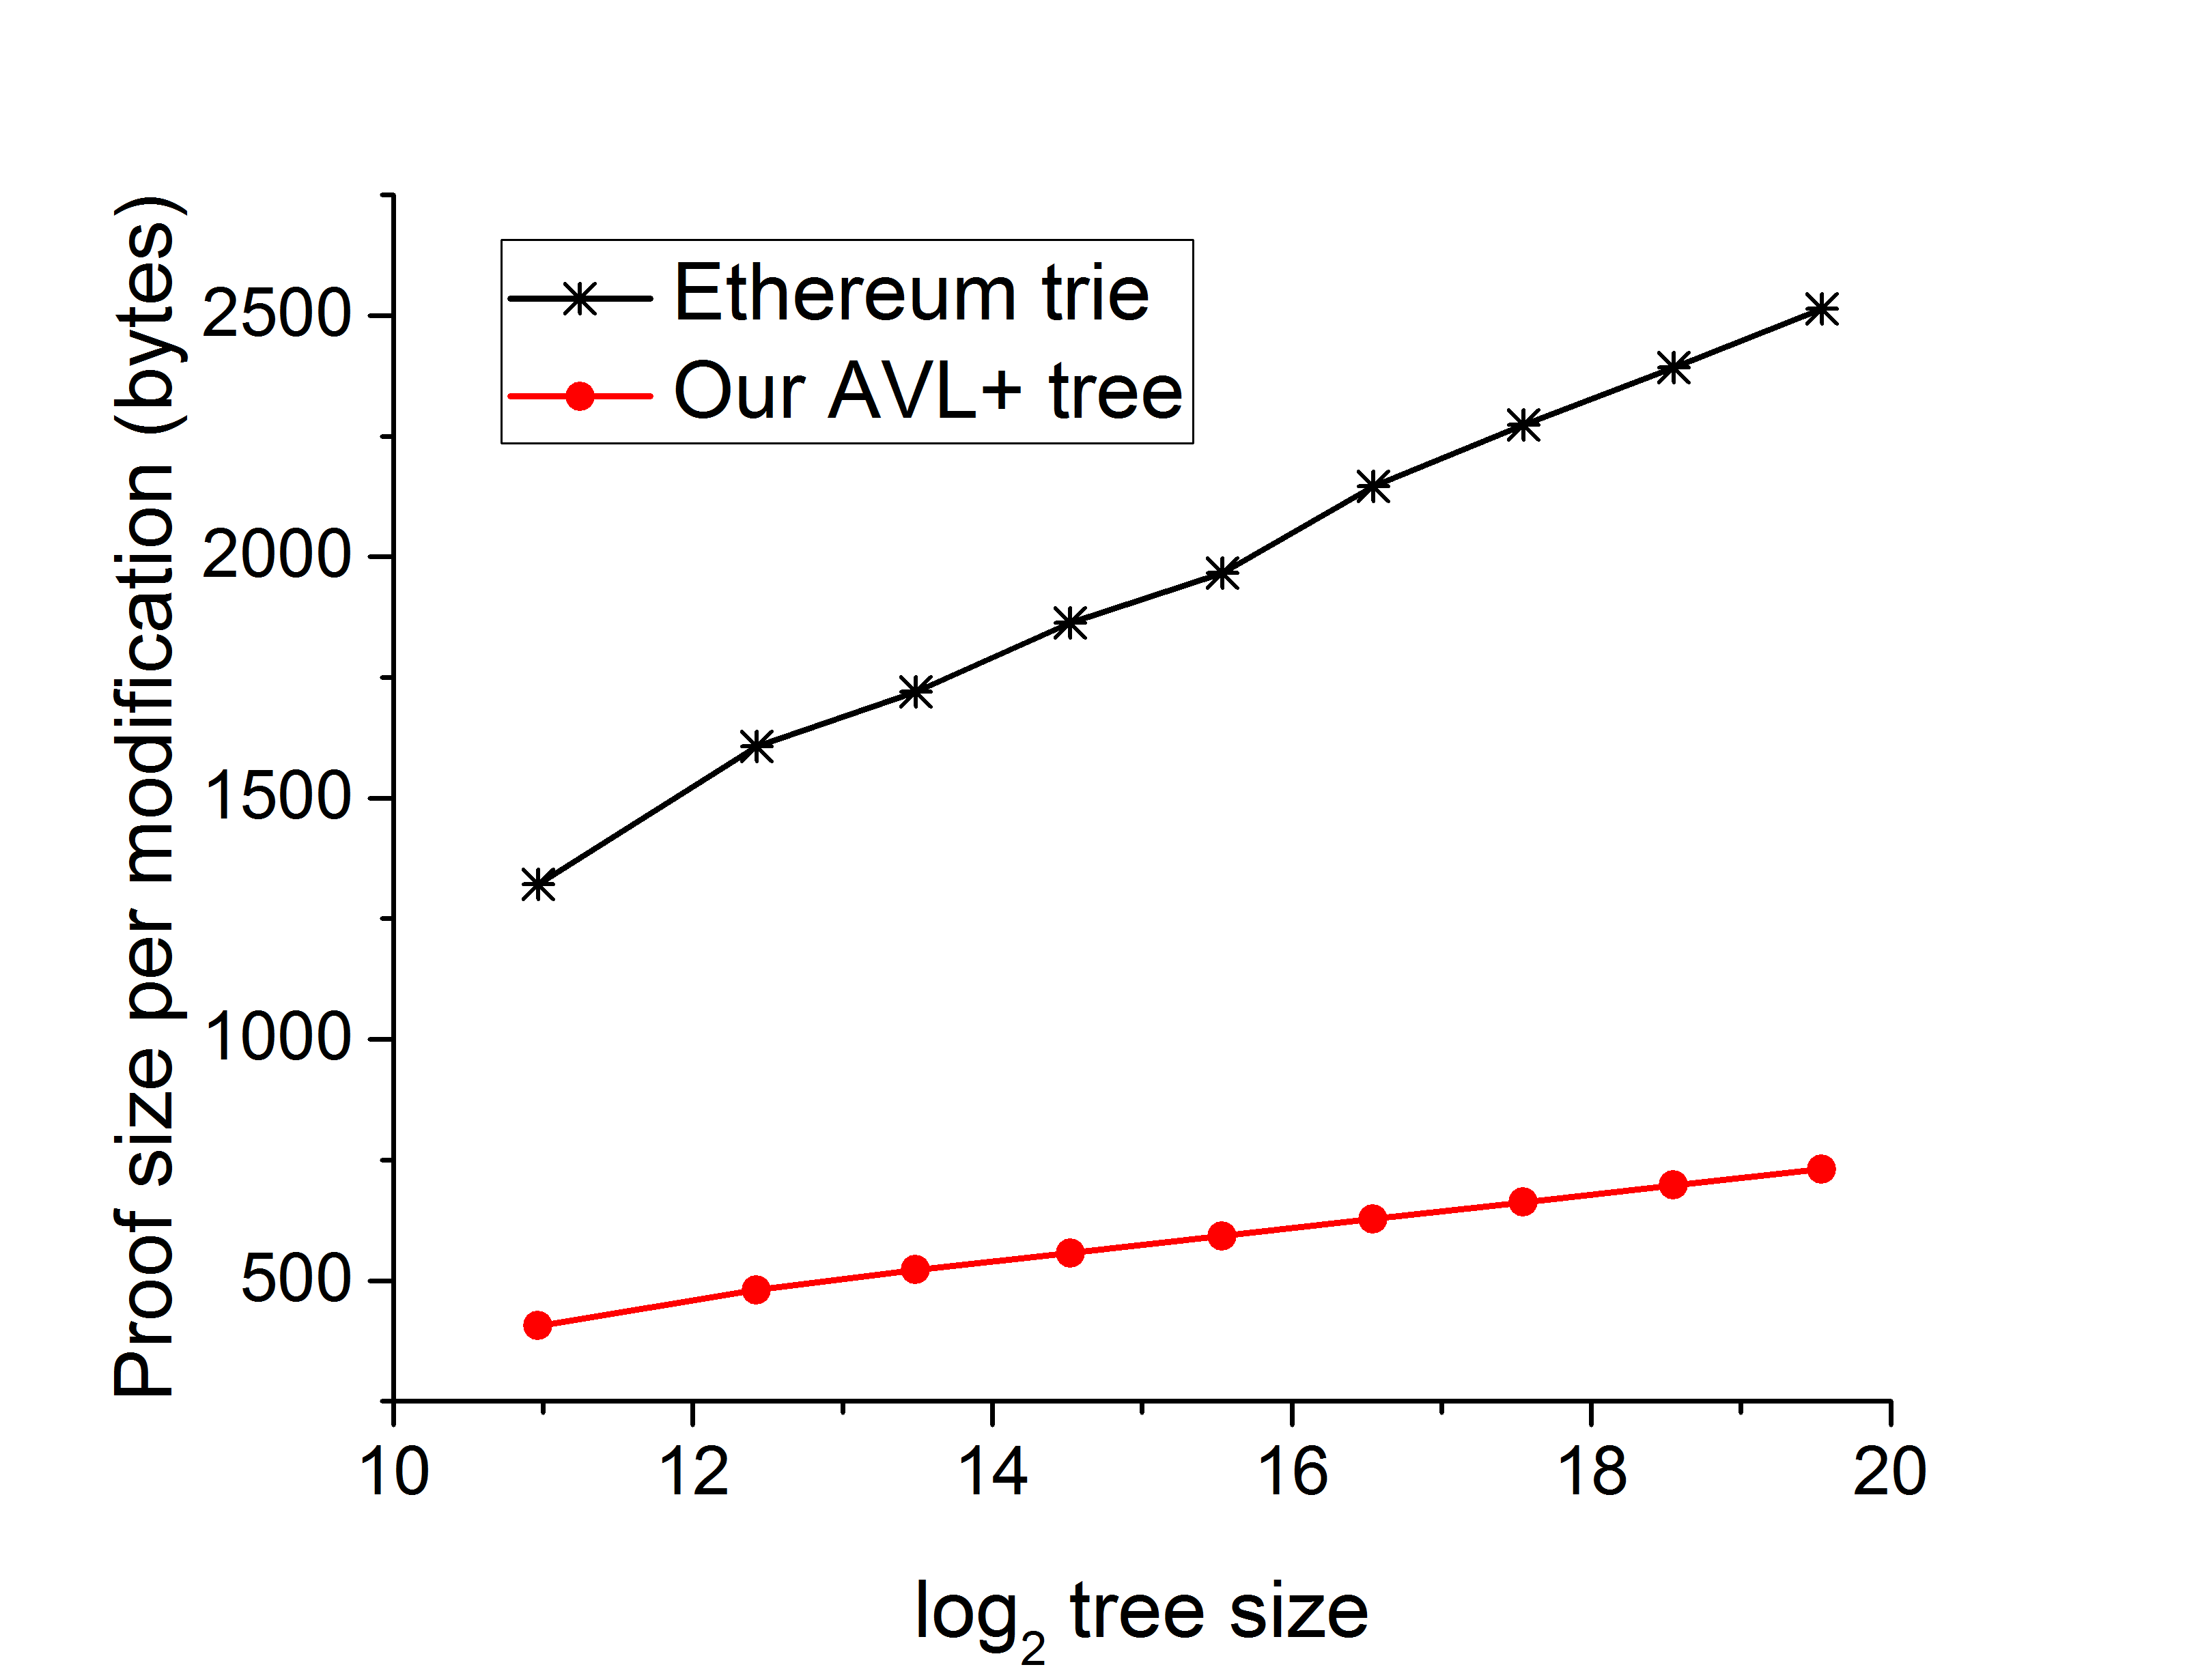
\includegraphics[width=0.5\textwidth]{img/proofSize.png}
    \caption{Proof size comparison with a Merkle patricia trie
    \label{fig:proofSize} }
\end{figure}

Finally, proofs for multiple transactions in a single block are compressed together, reducing their total length
by approximately an additional factor of 2:

\begin{figure}[H]
\begin{tabular}{cc}
\ifnum\lncs=0
\begin{minipage}{0.5\textwidth}
\else
\begin{minipage}{0.492\textwidth}
\fi
\begin{center}
\ifnum\lncs=0
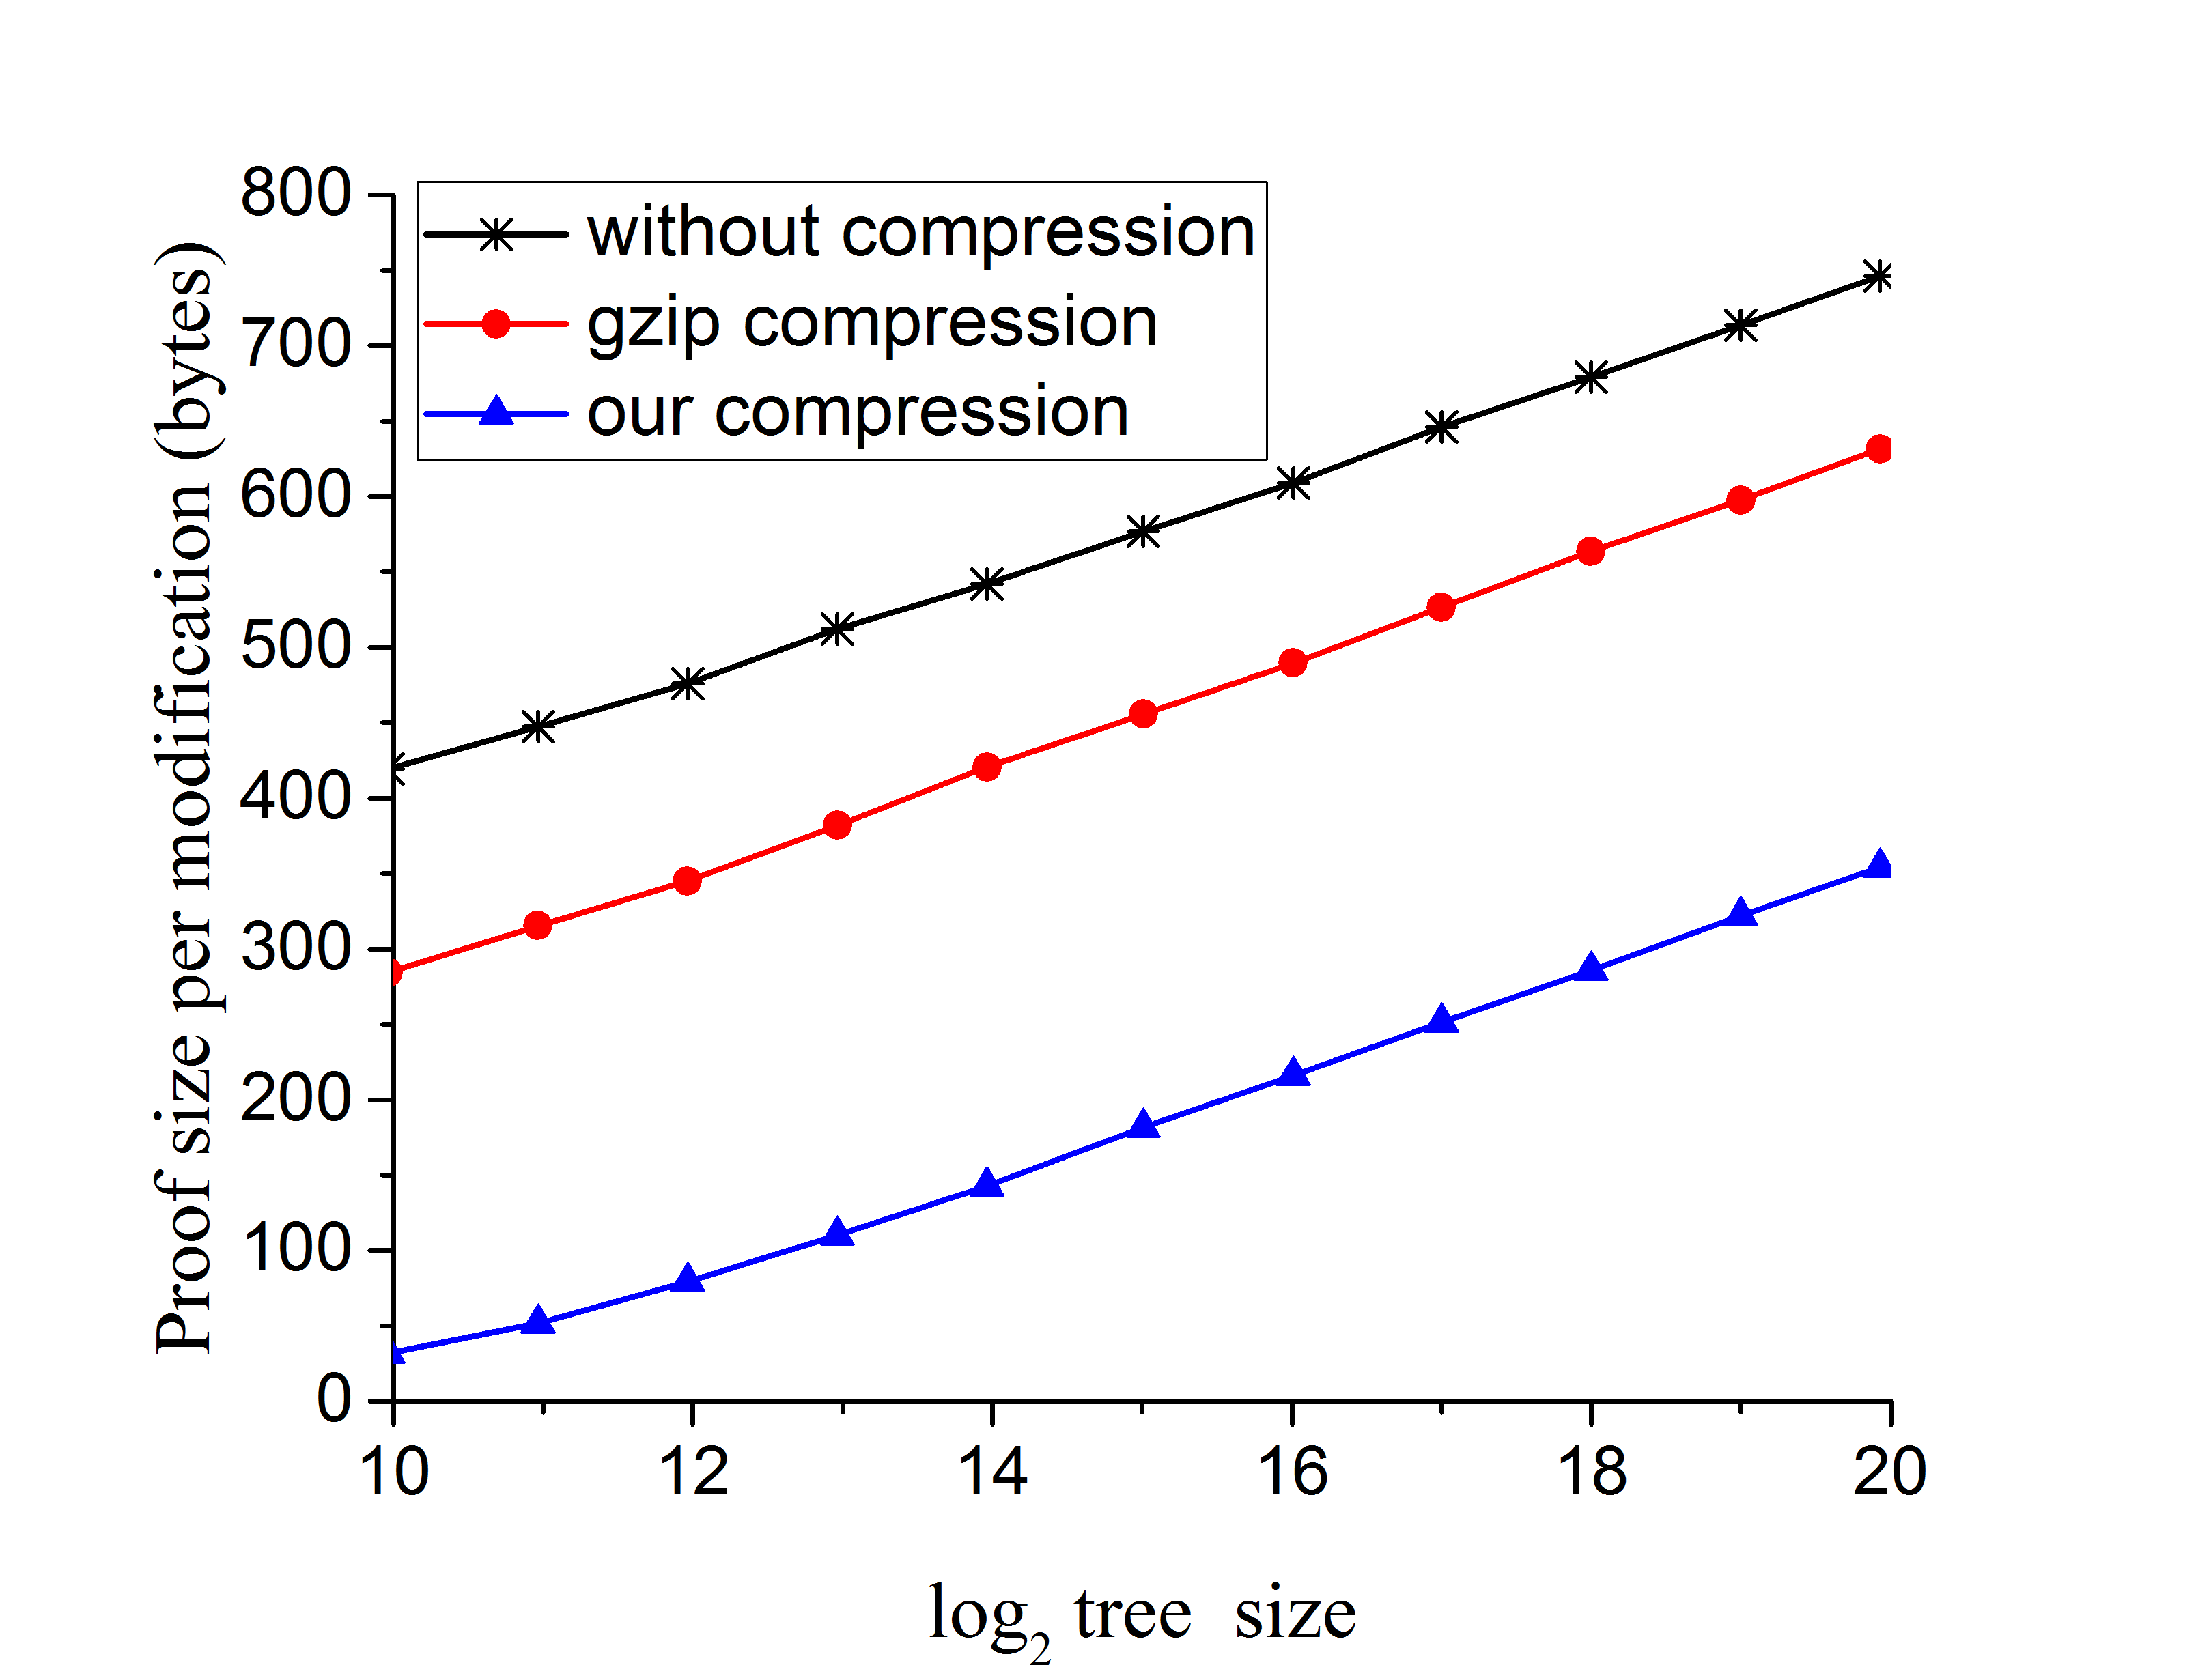
\includegraphics[trim={1.5cm 0cm 1.4cm 2cm},clip,width=\textwidth]{img/batching/proofSizeFromTreeSize.png}
\else
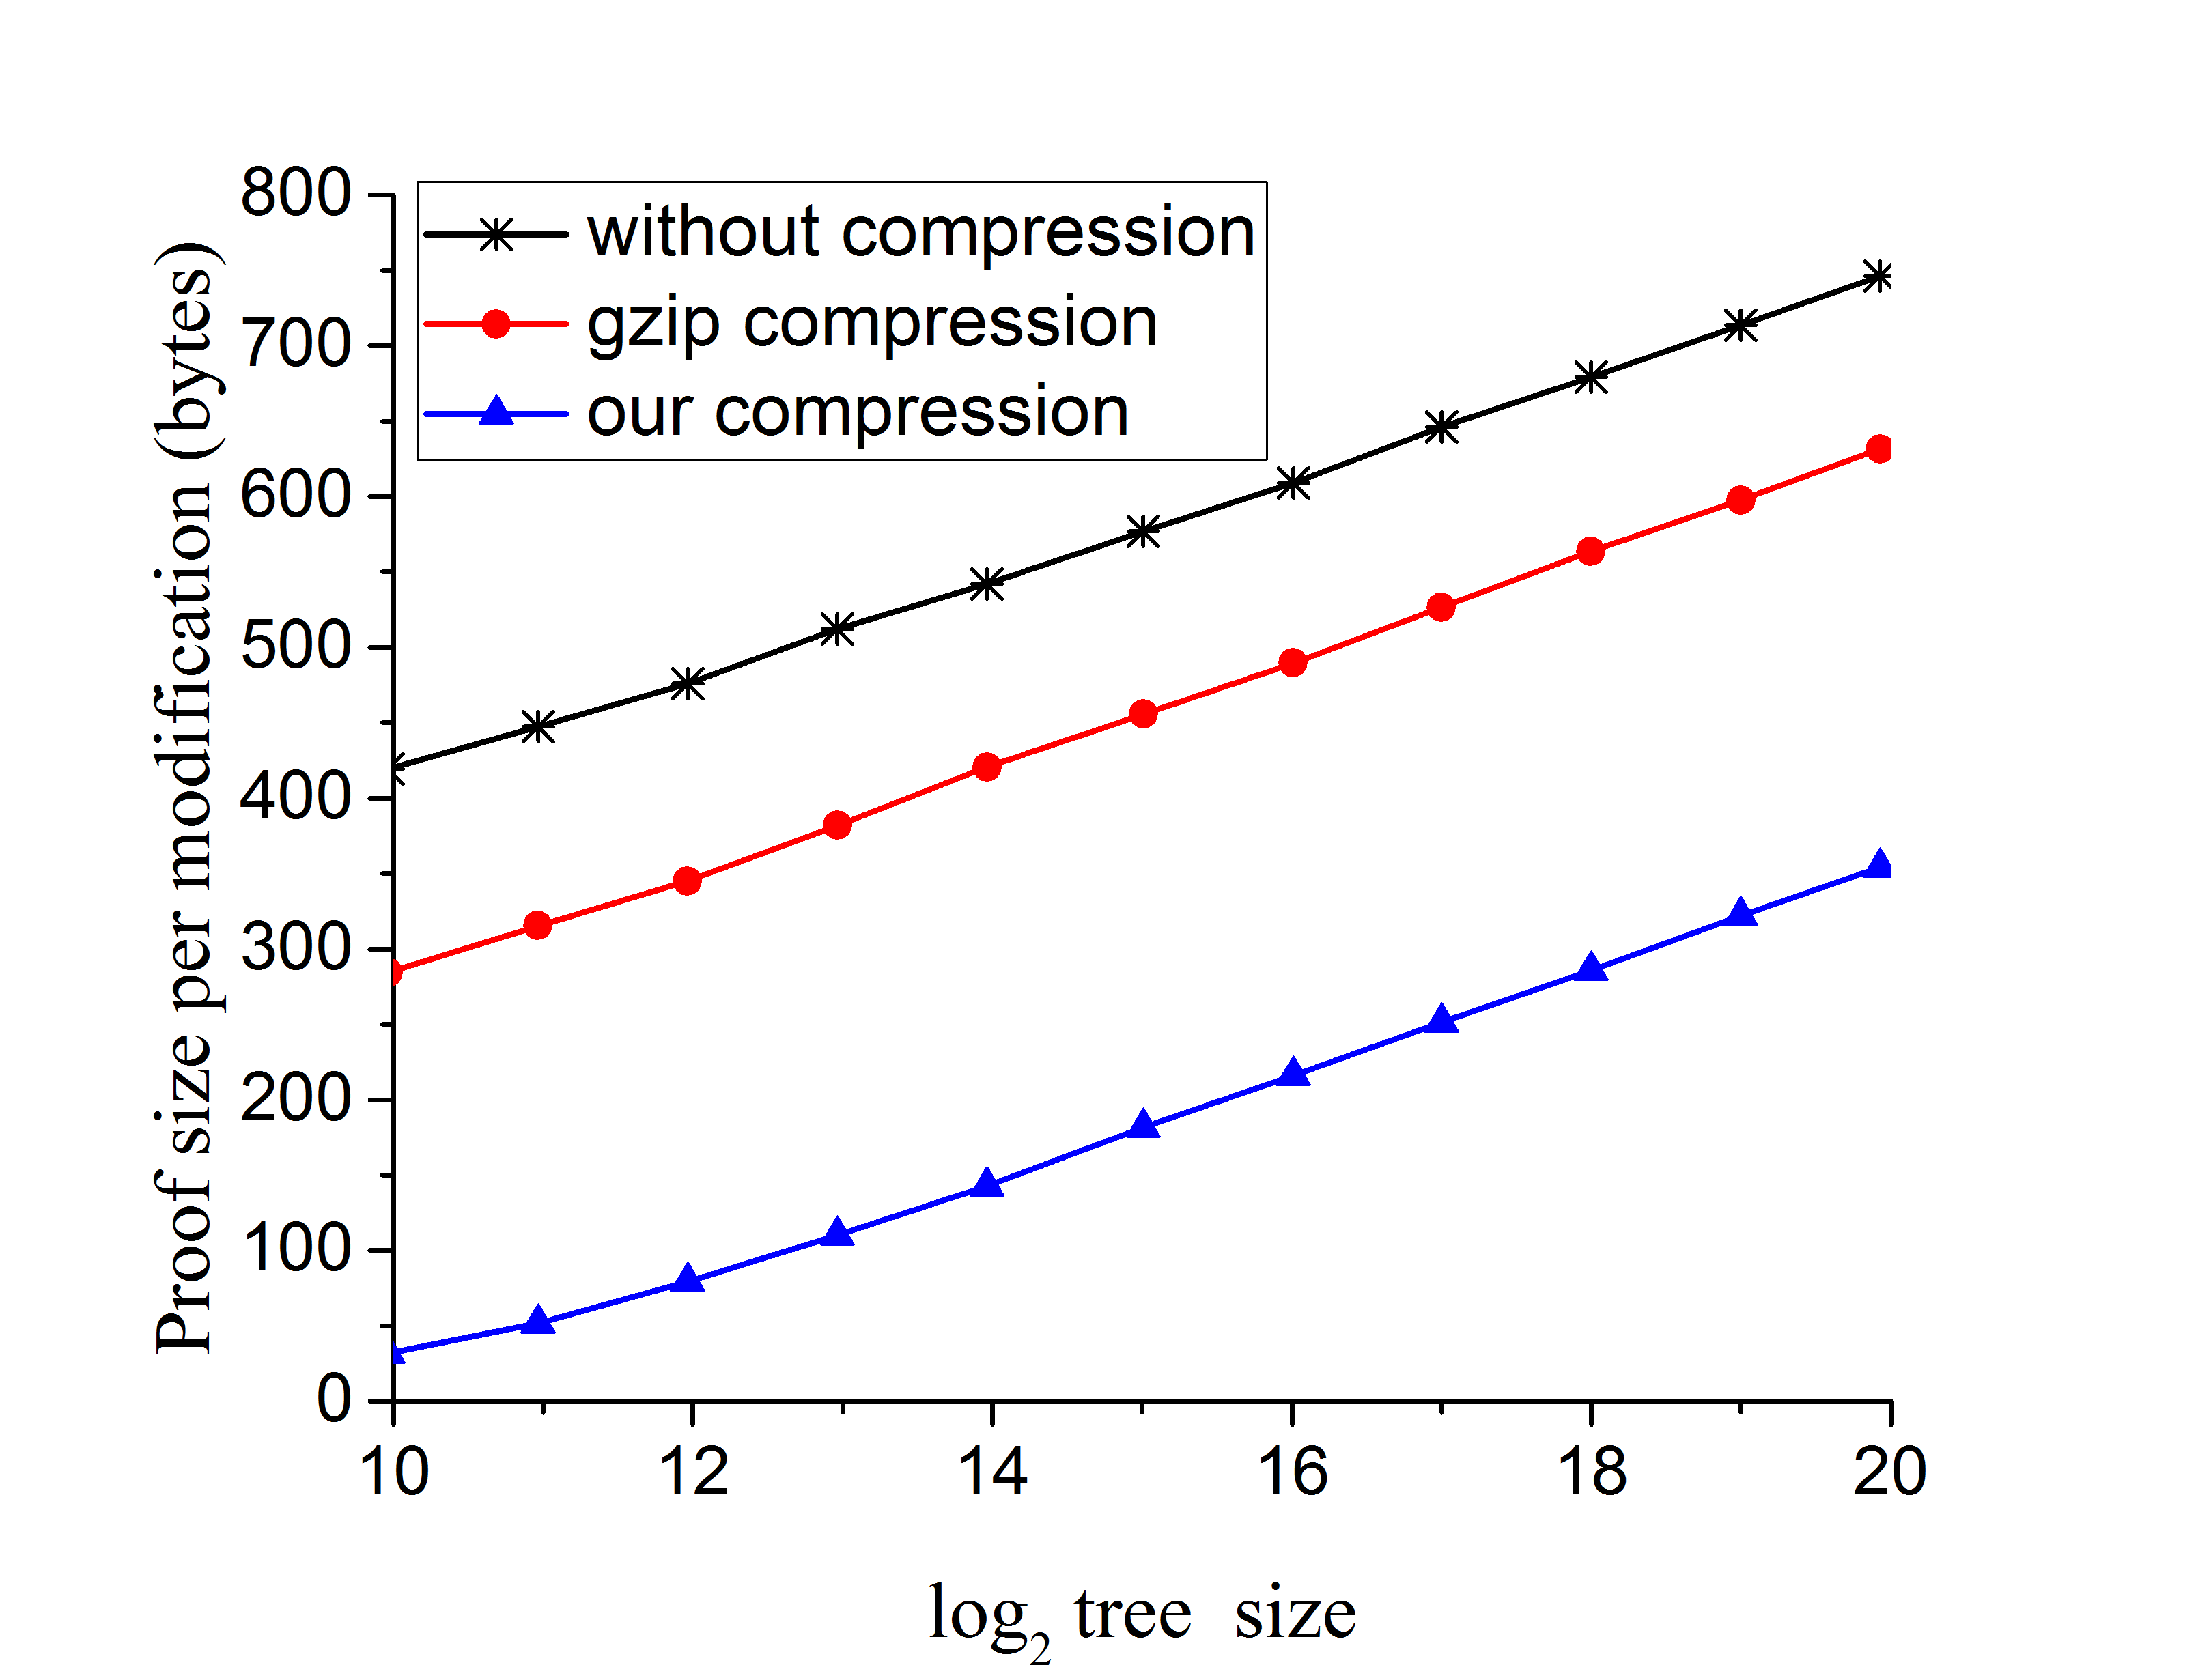
\includegraphics[trim={1.5cm 0cm 2cm 2cm},clip,width=\textwidth]{img/batching/proofSizeFromTreeSize.png}
\fi
\end{center}
\end{minipage}
&
\ifnum\lncs=0
\begin{minipage}{0.5\textwidth}
\else
\begin{minipage}{0.492\textwidth}
\fi
\begin{center}
\ifnum\lncs=0
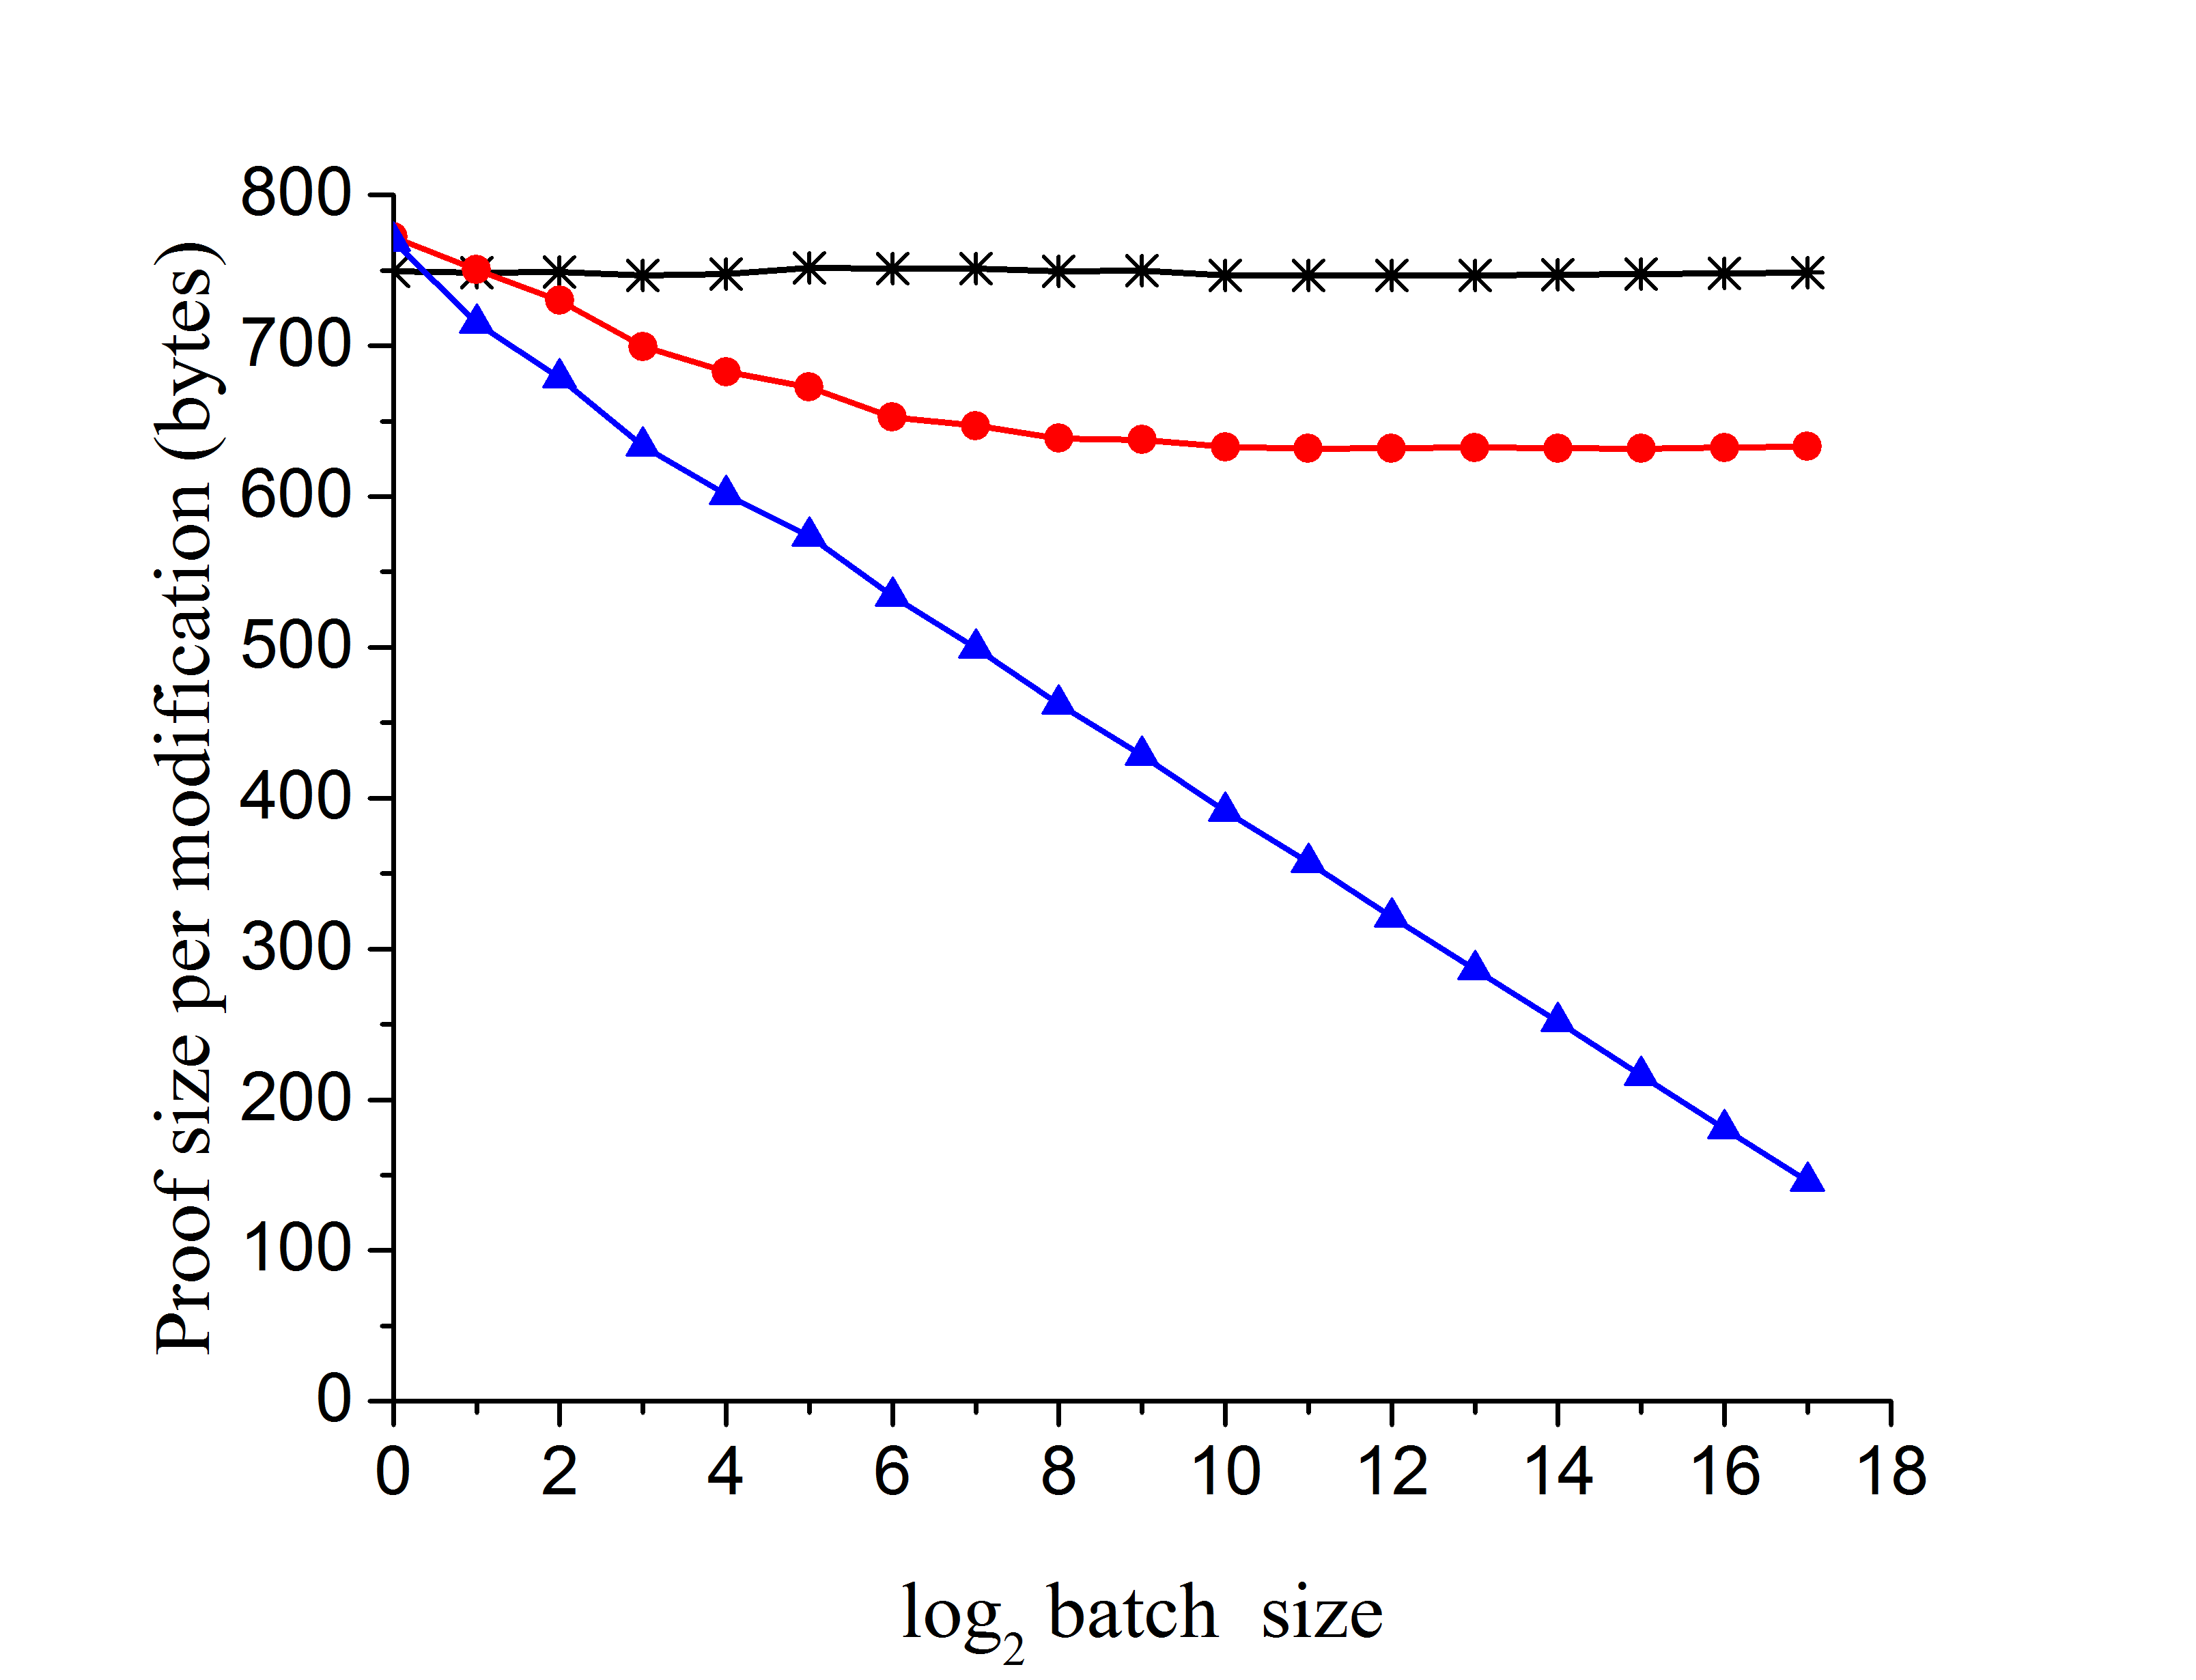
\includegraphics[trim={1.5cm 0cm 1.4cm 2cm},clip,width=\textwidth]{img/batching/proofSizeFromBatchSize2.png}
\else
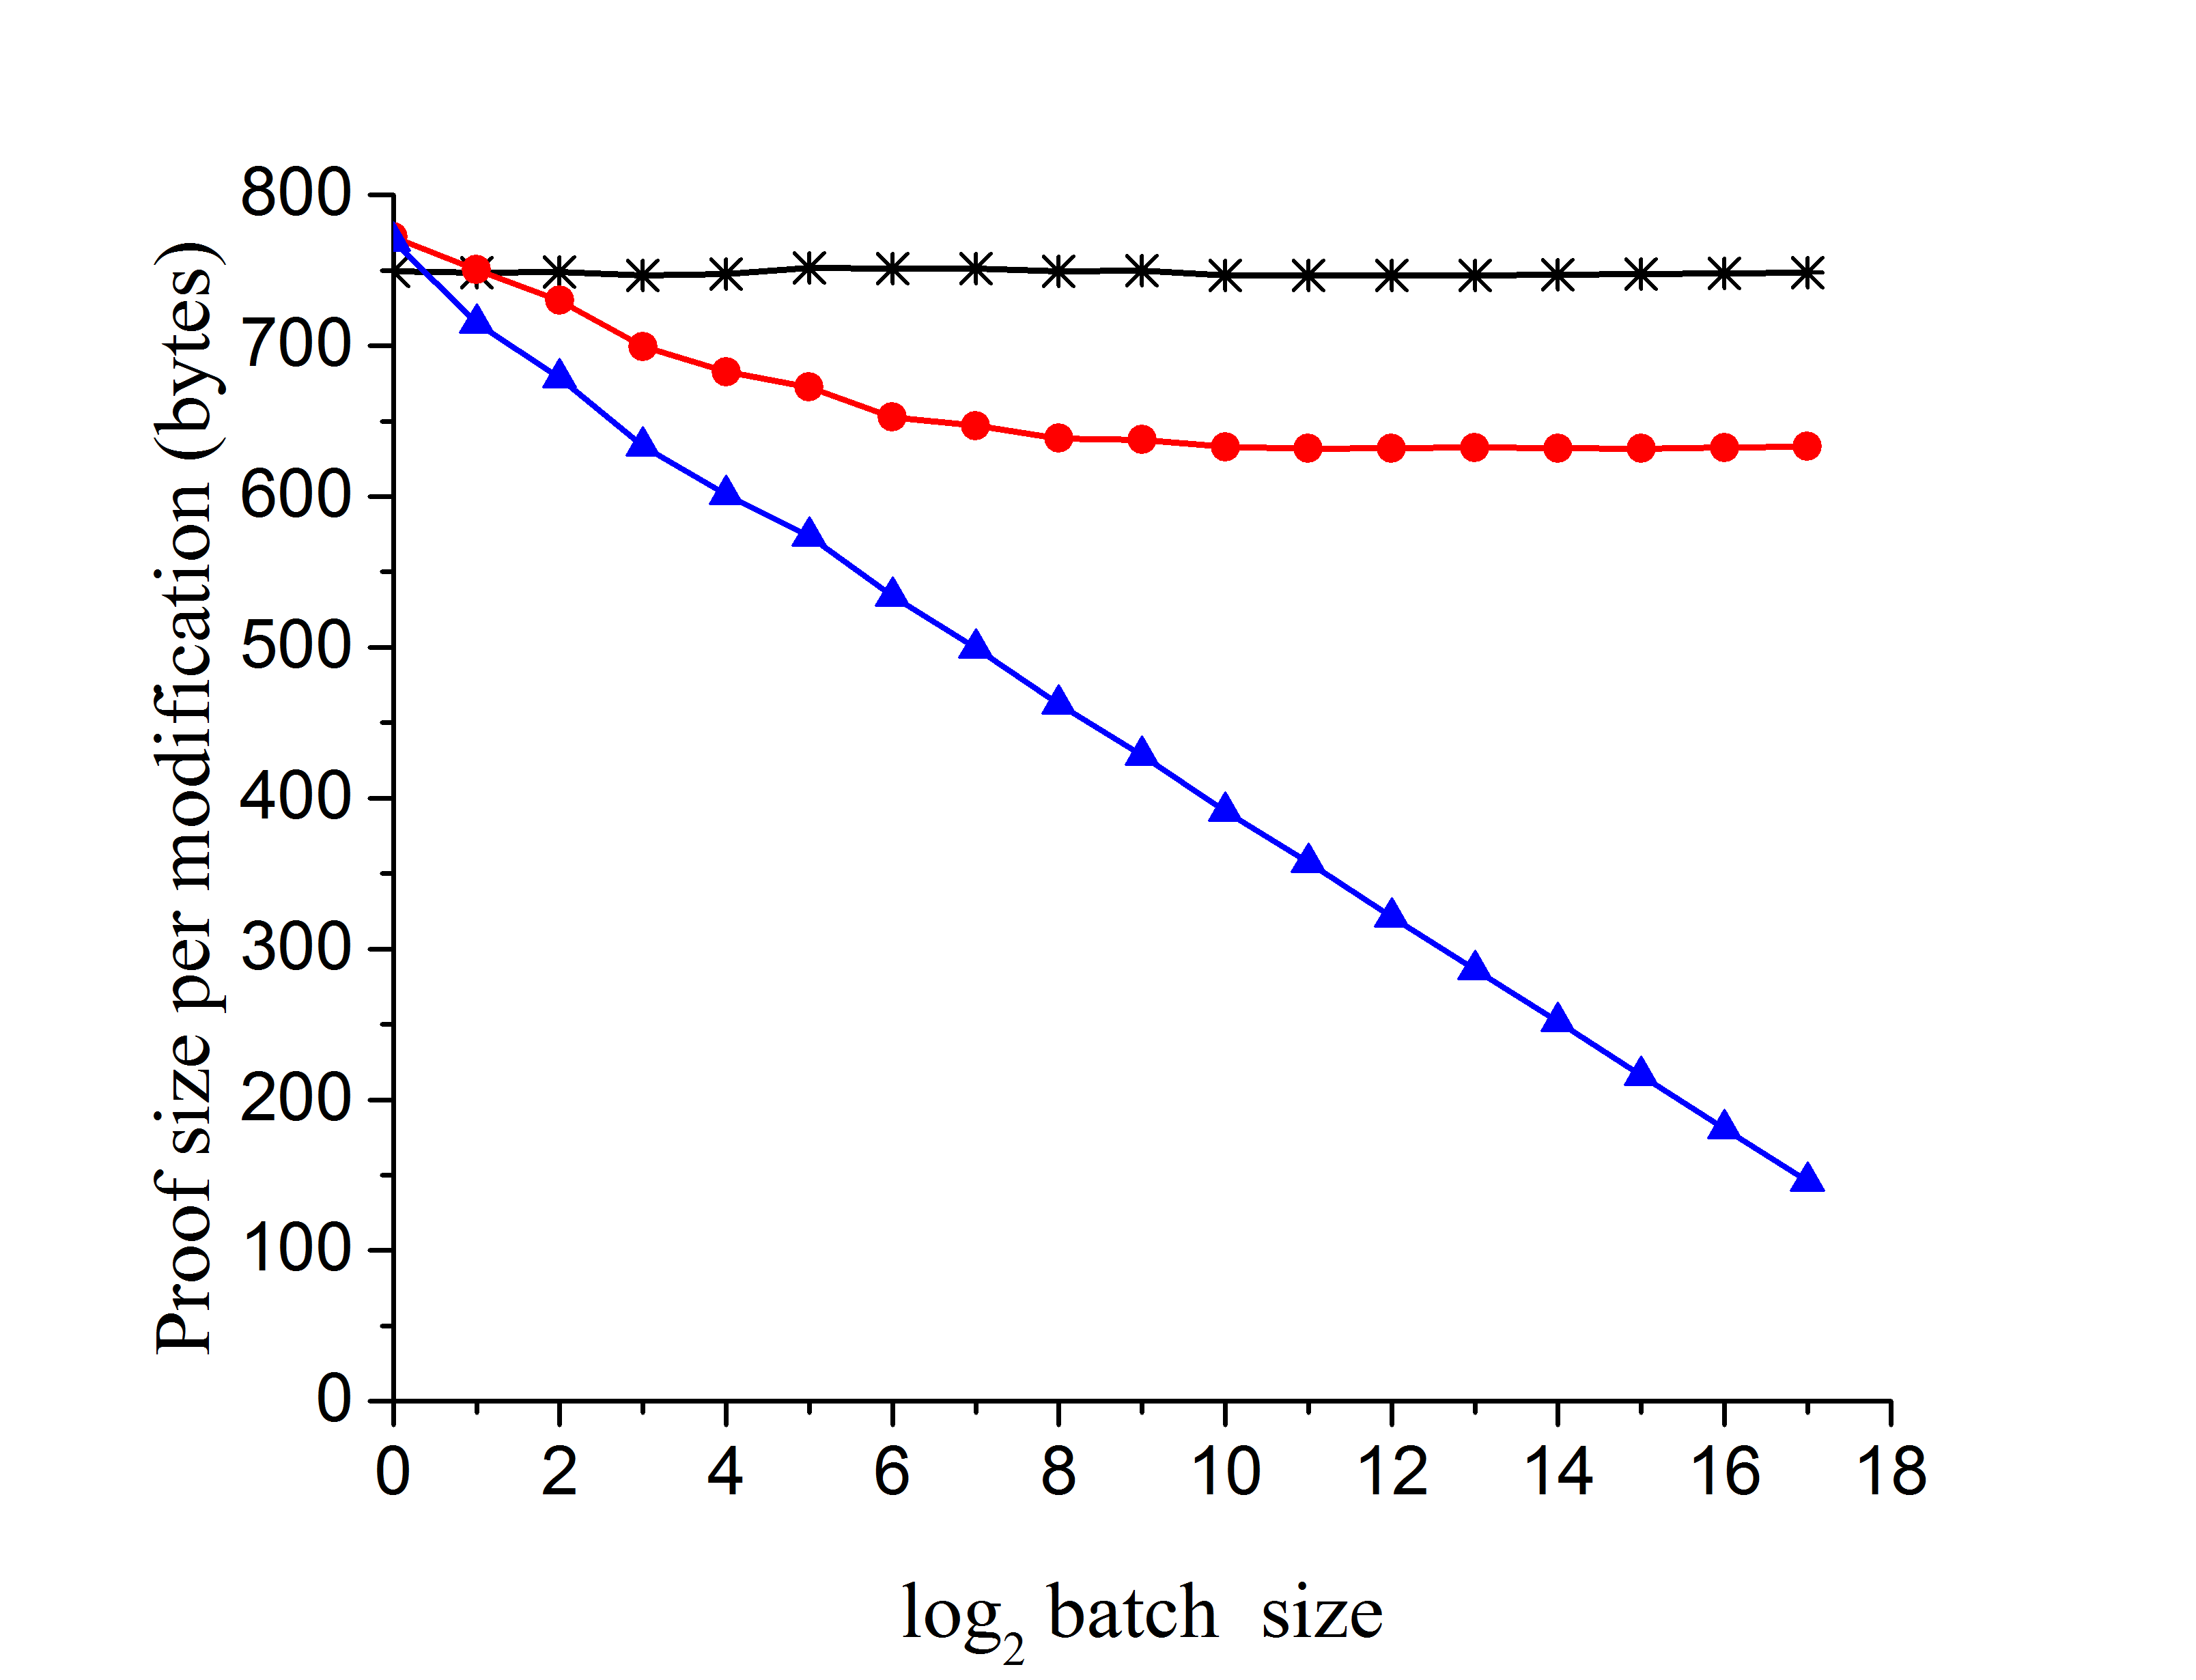
\includegraphics[trim={1.5cm 0cm 2cm 2cm},clip,width=\textwidth]{img/batching/proofSizeFromBatchSize2.png}
\fi
\end{center}
\end{minipage}
\end{tabular}
\caption{Left: proof size per modification for 2000 transactions as a function of starting tree size $n$.
Right: proof size per modification for a tree with $n = 1 000 000$ keys as a function of batch size $B$.
In both cases, half of the modifications were inserts of new (key, value) pairs and the other half were change of values for existing keys.}
\label{fig:batching}
\end{figure}


Thus, Ergo state provides an efficient and secure way to prove existence or non-existence of certain elements in
it, as well as proofs of tree modifications.
These tree operations are supported by the Ergo smart contract language, thereby providing the ability to implement sophisticated contracts like those discussed in Section~\ref{sec:contractual}.

